\section{Literature Review}

\subsection{Background}

\subsubsection{Neural Networks} \mbox{}\\

Neural networks can be traced back to 1943, when McCulloch and Pitts proposed a mathematical model of a biological neuron \cite{ideas_immanent_in_nervous_activity}. Rosenblatt extended this concept in 1958 with the introduction of the Perceptron \cite{perceptron}. The field did not see much progress until the 1980s, when the backpropagation algorithm was popularised \cite{backpropagation}. Finally, over recent years, advances in hardware capabilities have enabled neural networks to perform more complex tasks, leading to their adoption as state-of-the-art solutions across a wide range of applications, including medical diagnosis, autonomous driving, and image recognition.

More formally, a neural network can be seen as a feedforward, directed acyclic graph where each node, or neuron, performs an operation. \cref{fig:neural_network} illustrates a simple neural network, which can be divided into layers: the left-most is called the input layer, and the right-most is called the output layer. The layers that lie between the input and output layers are called hidden layers. Each node receives inputs, applies a transformation, and passes the result to subsequent nodes in the network.

To compute the output of a neural network, the input layer propagates the input $x$ forward through its successive layers $h$. At every stage, intermediate results are computed and passed to the next layer until the final output layer $\hat{y}$ is reached. This process is commonly referred to as forward propagation.

\begin{figure}[h]
\centering
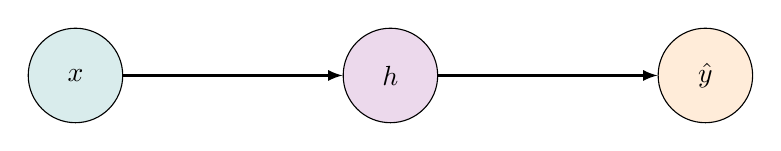
\begin{tikzpicture}[
    neuron/.style={circle, draw, minimum size=1.2cm, align=center},
    input/.style={neuron, fill=teal!15},
    hidden/.style={neuron, fill=violet!15},
    output/.style={neuron, fill=orange!15},
    arrow/.style={-latex, thick}
]

\node[input]  (x) at (0, 0)   {$x$};
\node[hidden] (h) at (4, 0)   {$h$};
\node[output] (y) at (8, 0)   {$\hat{y}$};

\draw[arrow] (x) -- (h);
\draw[arrow] (h) -- (y);

% Layer labels
% \node[below=0.3cm of x] {\small Input layer};
% \node[below=0.3cm of h] {\small Hidden layer};
% \node[below=0.3cm of y] {\small Output layer};

\end{tikzpicture}
\caption{A minimal neural network.}
\label{fig:neural_network}
\end{figure}


Since neural networks are graphs, there is no constraint regarding the number of nodes or layers they can contain. \autoref{fig:mlp} shows a neural network with 4 layers, each with 3 nodes. This type of neural network is called a multilayer perceptron (MLP).

\begin{figure}[h]
\centering
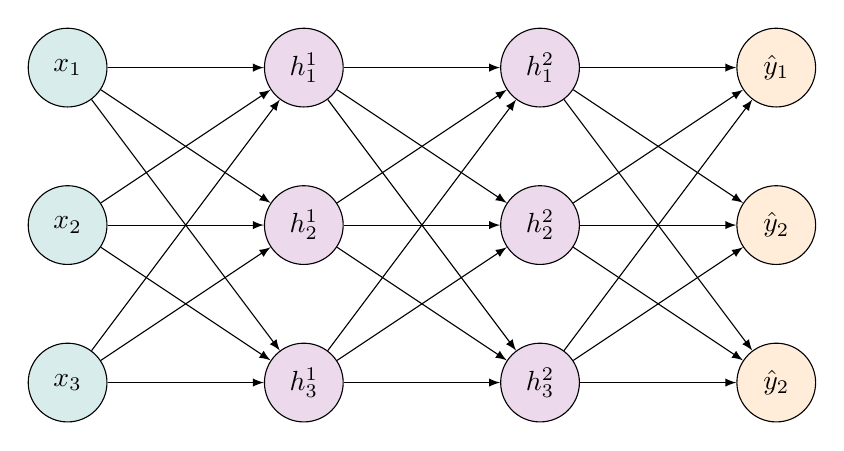
\begin{tikzpicture}[
    neuron/.style={circle, draw, minimum size=1cm, align=center},
    input/.style={neuron, fill=teal!15},
    hidden/.style={neuron, fill=violet!15},
    output/.style={neuron, fill=orange!15},
    arrow/.style={-latex, thick}
]

% Input layer neurons
\node[input]  (x1) at (0,  2)  {$x_1$};
\node[input]  (x2) at (0,  0)  {$x_2$};
\node[input]  (x3) at (0, -2)  {$x_3$};

% Hidden layer 1 neurons
\node[hidden] (h11) at (3,  2)  {$h_1^1$};
\node[hidden] (h12) at (3,  0)  {$h_2^1$};
\node[hidden] (h13) at (3, -2)  {$h_3^1$};

% Hidden layer 2 neurons
\node[hidden] (h21) at (6,  2)  {$h_1^2$};
\node[hidden] (h22) at (6,  0)  {$h_2^2$};
\node[hidden] (h23) at (6, -2)  {$h_3^2$};

% Output layer neurons
\node[output] (y1) at (9,  2)  {$\hat{y}_1$};
\node[output] (y2) at (9, 0)  {$\hat{y}_2$};
\node[output] (y3) at (9, -2)  {$\hat{y}_2$};

% Input to hidden layer 1 connections
\foreach \i in {1,2,3}{
    \foreach \j in {1,2,3}{
        \draw[-latex] (x\i) -- (h1\j);
    }
}

% Hidden layer 1 to hidden layer 2 connections
\foreach \i in {1,2,3}{
    \foreach \j in {1,2,3}{
        \draw[-latex] (h1\i) -- (h2\j);
    }
}

% Hidden layer 2 to output connections
\foreach \i in {1,2,3}{
    \foreach \j in {1,2,3}{
        \draw[-latex] (h2\i) -- (y\j);
    }
}

% Layer labels
% \node at (0,  -3.2) {\small Input layer};
% \node at (3,  -3.2) {\small Hidden layer 1};
% \node at (6,  -3.2) {\small Hidden layer 2};
% \node at (9,  -3.2) {\small Output layer};

\end{tikzpicture}
\caption{A Multilayer Perceptron.}
\label{fig:mlp}
\end{figure}


Neural networks can be modelled as mathematical functions that map a set of real-valued inputs to real-valued outputs. Formally, a neural network can be defined as:
\[
N : \mathbb{R}^{k_I} \rightarrow \mathbb{R}^{k_O}
\]
where $k_I$ and $k_O$ denote the dimensions of the input and output spaces, respectively. The input is represented as a vector $x_I = (x_1, \ldots, x_{k_I})$, and the output as $x_O = (y_1, \ldots, y_{k_O})$.

Each layer in a neural network performs a two-step computation: a linear transformation followed by a non-linear activation function. More specifically, given an input vector, each layer applies a weighted sum combined with a bias term, and then passes the result through a non-linear function such as the Rectified Linear Unit (ReLU). This layered structure enables neural networks to approximate complex, non-linear functions.

\subsubsection{DNNs} \mbox{}\\

The term \textbf{Deep} in \textit{Deep Neural Networks} refers to networks that contain a large number of hidden layers. Deeper networks can learn more complex representations of the input. However, this increase in capability comes at the cost of interpretability. DNNs are often considered \textit{black-box} models, as their internal inference process is not interpretable by humans. As a result, undesirable behaviour may remain hidden within the network. This concern has reflected negatively on their adoption in safety-critical applications \cite{interpretable_machine_learning}.

\subsubsection{DNN Verification} \mbox{}\\

% NOTE: Why do we need to prove DNNs?
Even though the idea of verifying Neural Networks has been studied since the early days of AI, the necessity to prove them correct did not arise until recent days. This is because it was shown that DNNs could carry out tasks that were technically unfeasible before their arrival. As a result, the use of DNNs in safety-critical domains increased rapidly (e.g., in self-driving cars and surgical procedures). As a consequence, the necessity to ensure robustness, safety, and consistency also increased.

% NOTE: Why can't DNN be verified as normal software
Modern feedforward DNNs often process inputs consisting of thousands of elements, and may operate on multidimensional data such as images or other structured representations. In traditional software, empirical approaches such as testing, that is, verifying the output for a finite set of inputs, are widely used due to their simplicity and scalability in order to guarantee a certain level of correctness. However, the size of the input space in DNNs makes this approach infeasible.

Consider, for example, a DNN trained to detect the presence of a vehicle in an image: one valid input might be the image shown in \autoref{fig:autonomous-driving-pixels}. A visually identical input, but with slightly altered pixel brightness, is shown in \autoref{fig:autonomous-driving-altered-pixels}. In both cases, the DNN should yield the same result: a positive classification. But, since each image have different brightness values, there is no guarantee they will do so. This illustrates why exhaustive testing cannot guarantee correctness, since the space of possible inputs is too large to be fully explored.

\begin{figure}[h]
    \centering
    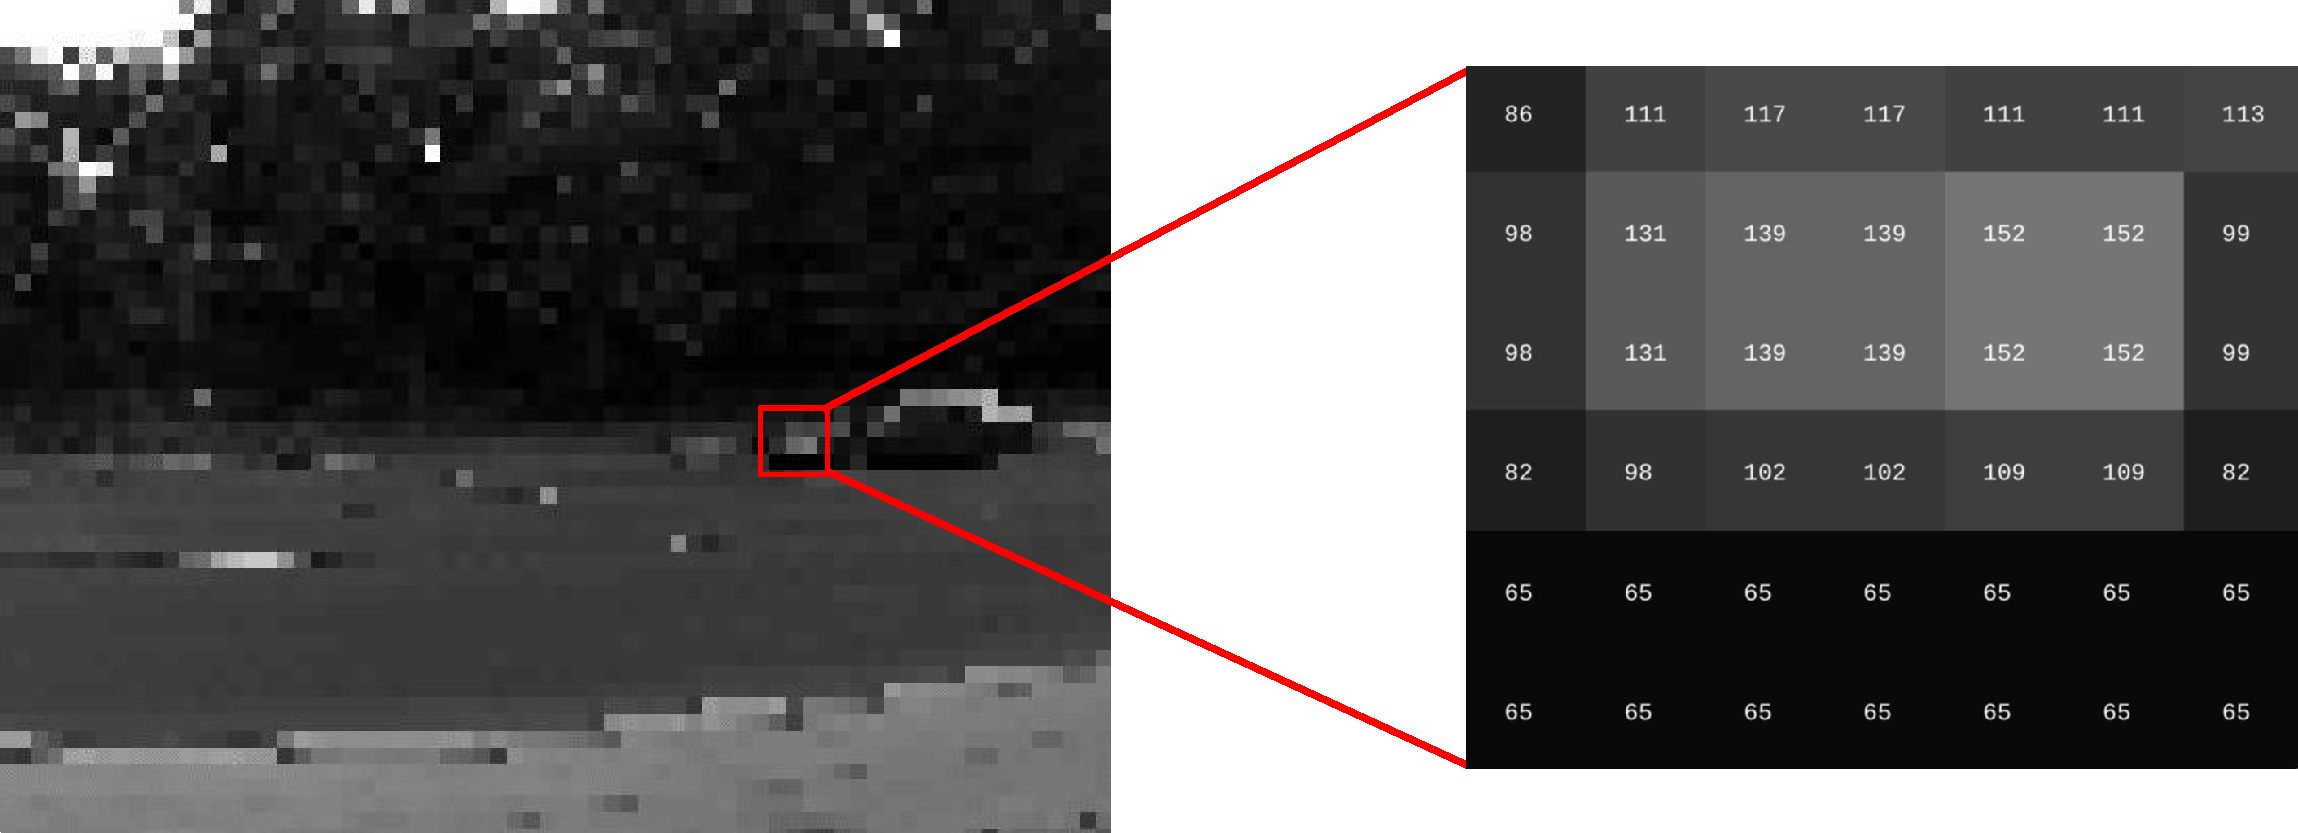
\includegraphics[width=\textwidth]{images/autonomous_driving_pixels.pdf}
    \caption{Autonomous driving input with zoomed pixel values.}
    \label{fig:autonomous-driving-pixels}
\end{figure}

\begin{figure}[h]
    \centering
    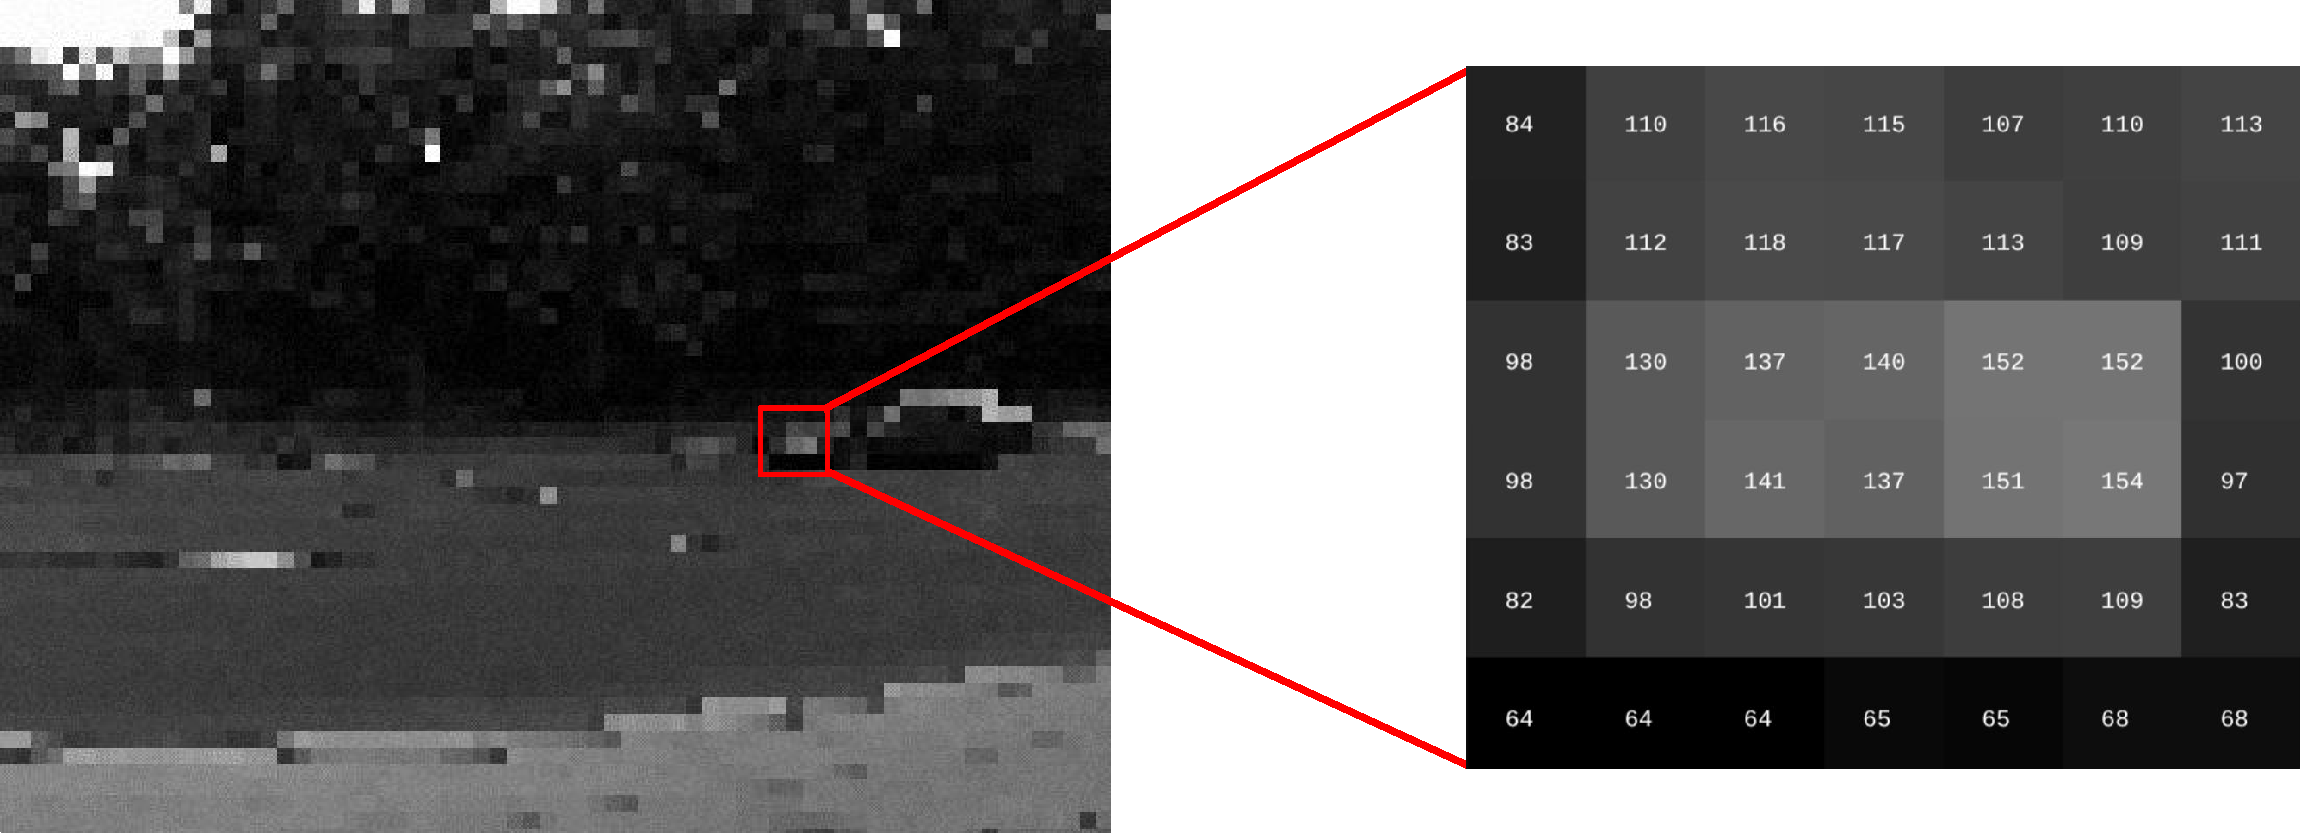
\includegraphics[width=\textwidth]{images/autonomous_driving_altered_pixels.pdf}
    \caption{Slightly altered autonomous driving input with zoomed pixel values.}
    \label{fig:autonomous-driving-altered-pixels}
\end{figure}


Formal verification addresses the already stated concern by providing mathematical guarantees about the behaviour of a DNN. Rather than sampling a finite set of inputs, it reasons over entire regions of the input space, ensuring that any input within a defined region will map to an output within a defined region.

In order to formally define a neural network verification problem, the following components are required:
\begin{itemize}
    \item A \textbf{pre-condition} (or input specification), defining the set of admissible inputs.
    \item A \textbf{post-condition}, specifying the desired property of the outputs.
    \item A \textbf{neural network} $N$, representing the function under analysis.
\end{itemize}

DNN verification methods can be broadly classified into complete and incomplete approaches \cite{algorithms_for_verifying_dnns}. Both are sound, meaning that if the algorithm reports that a property holds, it is guaranteed to do so. Complete approaches additionally guarantee that if a property holds, the algorithm will always detect it. Incomplete approaches, by contrast, may fail to verify a property even when it holds, as they rely on over-approximations that can be overly conservative.

Orthogonally, DNN verification techniques can also be categorised into
constraint-based and abstraction-based approaches \cite{introduction_to_nn_verification}.

\paragraph*{Constraint-based Verification.} The verification encodes
the DNN verification problem as a logical satisfiability problem. The network,
including its weights, biases, and activation functions, is encoded as a set of
constraints alongside the pre-condition and post-condition. The verifier then
determines whether there exists an input that satisfies the pre-condition but
violates the post-condition. If no such input exists, the property is guaranteed
to hold.

\paragraph*{Abstraction-based Verification.} The verification addresses
the scalability limitations of constraint-based methods by over-approximating the
set of reachable values through the network, rather than reasoning about exact
values. Instead of encoding the network as a set of constraints, it represents
sets of possible inputs and outputs as geometric shapes, and propagates them
through the network layer by layer.

\subsubsection{SMT Solvers} \mbox{}  \\

% NOTE: What are SMT Solvers
An SMT solver is a tool for determining whether a set of logical formulas is satisfiable. This means whether there exists a set of values for variables for which all logical formulas are true. It is an extension of SAT solvers that can only handle Boolean variables. However, SMT solvers can handle background theories such as linear arithmetic, arrays, bit vectors, and more. This enables more expressive solvers and can be applied to real-world applications.

% NOTE: Why are SMT Solvers useful
For DNN verification, SMT solvers are used to translate the DNN, including its weights, biases, and activation functions, into a set of arithmetic constraints, along with the pre-condition and post-condition. The solver attempts to find an input that satisfies the pre-condition but fails to satisfy the post-condition. If no such input exists, then it is verified that the property holds. If a counterexample is found, then it is used to prove that the property does not hold. One of the most prominent SMT solvers is Z3 \citet{z3} . DNN-specific solvers such as Marabou extend these ideas with optimisations for DNNs.

\subsubsection{Marabou} \mbox{} \\

Marabou is an SMT, constraint-based DNN verifier that answers queries over networks. Marabou performs satisfiability checking based on an input query, which is compromised by set properties that specify the property to be checked, a neural network, and a set of linear and non-linear constraints.
\vspace{0.5cm}

Marabou's architecture can be split into components and sub-components:
\paragraph*{Front end.} The front end module provides a way of supplying all the information required to determine the satisfiability of the DNN to the back end, without explicitly interacting with it.
\paragraph*{Back end.} The back end module's main role is to perform all operations related to DNN verification, from reasoning about the satisfiability of the input query to generating proof certificates. It is comprised of multiple components:
\paragraph*{Engine.} The engine module's job is to determine the satisfiability of the DNN against the input query.
\paragraph*{Proof module.} The proof module provides a way of generating proof certificates once a problem is classified as UNSAT.
\paragraph*{Context-Dependent Data-Structures.} These data structures store verification-related data that can be retrieved and reused at later stages of the verification process.

\vspace{0.5cm}

Internally, Marabou's engine follows a set of steps to determine
whether an input query is satisfiable:

\begin{enumerate}
    \item \textbf{Encoding.} The input query, comprising the neural network, the input constraints, and the property to verify, is encoded as a system of linear and non-linear constraints.
    \item \textbf{Linear reasoning.} Simplex \cite{calculus_of_computation} is applied to reason about the linear constraints. If a satisfying assignment is found at this stage, the answer is SAT, and the assignment serves as a counterexample witnessing the violation of the property.
    \item \textbf{Case-splitting.} When a non-linear constraint is encountered, such as a ReLU activation, Marabou performs case-splitting, dividing the problem into two sub-problems, one for each regime. Each sub-problem is handed back to Simplex.
    \item \textbf{Recursive search.} Steps 2 and 3 are applied recursively to each sub-problem until every branch is resolved as either SAT, where a satisfying assignment is found, or no solution is found, which implies UNSAT, and a proof certificate is generated.
    \item \textbf{Conclusion.} If every branch of the search tree is determined to be UNSAT, Marabou concludes that no satisfying assignment exists for the entire query. The Farkas certificates from all branches are combined into a proof tree, which a proof checker can then validate.
\end{enumerate}

Once the engine has concluded that the input query is UNSAT using the above process, the proof module is responsible for generating a proof certificate. This certificate consists of a proof tree, which mirrors the case-splitting structure generated by the engine. The nodes in the tree consist of the splits generated during the case splitting process. The leaves in the tree correspond to the branches in the case-splitting process that were marked UNSAT by the Simplex procedure. These leaves also include a Farkas vector, a set of coefficients. These coefficients serve to witness the UNSATness of the constraints in the branches. The root in the tree represents the original input query. This tree represents a complete record of the absence of a satisfying assignment.

\subsubsection{Interactive Theorem Provers} \mbox{} \\
Interactive Theorem Provers (ITPs), also known as interactive proof assistants, are computer tools designed to help users develop formal proofs, which are then verified by the system. ITPs differ from automated theorem provers, whose main objective is to resolve formal proofs without user interaction automatically. ITPs, on the other hand, require continuous human involvement and guidance. ITPs are best used when proving complex theorems, which automated theorem provers cannot reason about.

\textbf{Imandra} is a powerful ITP and automated reasoning system. Imandra uses a purely functional subset of OCaml. Imandra combines automated reasoning and interactive theorem proving. This means many proofs will be automatically discharged without the user having to interact with the system. Imandra has been used in the development of several verification projects in industry and academia.

\textbf{Rocq} (previously known as Coq) is a popular open-source ITP. Rocq's foundation lies in the Calculus of Inductive Constructions (CIC). This is a dependent type system in which types depend on values. This allows the user to express precise formal statements in the type system. Rocq has been used across a wide range of academic projects. These projects include the formalisation of the Four Colour Theorem and the CompCert verified C compiler \citep{compcert_rocq}.

\subsection{Related Work}

\subsubsection{ITP Neural Network Verification} \mbox{} \\

The topic of formally verifying neural networks is very broad, meaning there is no single established procedure for how to proceed. Even though in our work we focus on DNN verification coupled with proof checking in Rocq, there have been approaches that fit an entire neural network into Rocq to prove a property of it \cite{formally_verified_nn_converter}.

\subsubsection{Proof Production} \mbox{} \\

Even though the idea of proof production has been conceived since the late 1990s \citep{proof_carrying_code}. The first appearance of proof production in the DNN verification field did not occur until the development of \citet{nn_proof_production}, which adopted a proof production approach to ensure the absence of errors in the results. Since then, new developments have emerged, such as the approach of minimising irrelevant information from the proof certificates generated by a DNN verifier \citet{proof_minimization_in_nn_verification}.


\subsubsection{A Certified Proof Checker for Deep Neural Network Verification in Imandra} \mbox{} \\

\citet{certified_proof_checker} presents a fully certified proof checker implemented in Imandra. The novelty of the implementation relies on the usage of the re-adapted Farkas lemma, which purpose is to certify that a system of linear constraints  has no solution, for solving DNN verification proposed by \citet{lp_foundations_an__extensions}

\subsection{Critical Analysis}

Although there is a clear and progressive trajectory in the literature towards certified DNN verification, several challenges remain before the field can transition from a predominantly academic research area to an industry-ready technology. In particular, current approaches still struggle with scalability, and the limitations identified in the literature continue to motivate the development of the proposed project.



% TODO: Talk about ITPs and DNN Verification

\newpage
